\chapter{Implementacja}
W ramach pracy powstała biblioteka zawierająca moduły ułatwiające implementację protokołów działających w ramach WSN. Stanowi ona rozszerzenie biblioteki INET, zawierającej moduły dla standardu IEEE 802.15.4.

Biblioteka składa się z następujących modułów:
\begin{itemize}
	\item WSNNode --- złożony moduł ,,abstrakcyjny'' stanowiący bazę dla węzłów sieci. W jego skład wchodzą:
\begin{enumerate}
\item Moduły pochodzące z biblioteki INET:
\paragraph{Moduł mobilności} Jest to moduł zarządzający położeniem oraz mobilnością węzła. Jako, że zakres pracy obejmuje węzły stacjonarne, jako wartość domyślna został przyjęty moduł StationaryMobility, który jedynie śledzi położenie węzła.
\paragraph{Źródło energii} Jako źródło energii wykorzystany został udostępniony przez Inet moduł prostego zasobnika energii (SimpleEnergyStorage).
\paragraph{Tablica interfejsów} Przechowuje informacje o interfejsach danego węzła. W przypadku objątych tą pracą symulacji jest to jeden interfejs radiowy.
\paragraph{Moduł karty sieciowej} Jest to moduł symulujący kartę sieciową. Zawiera się w nim moduł odpowiadający za warstwę fizyczną oraz moduł łącza danych.
\paragraph{Moduł stanu węzła} Jest to moduł informujący o aktualnym stanie węzła.
\item Moduły stworzone w ramach pracy dyplomowej:
\paragraph{Moduł monitora} Jest to autorski moduł monitorujący poziom energii w węźle do celów statystycznych. Moduł w regularnych odstępach czasu emituje sygnał zawierający aktualną ilość energii w węźle. Zadanie to realizuje funkcja \textit{updateStoredEnergy()}.
\begin{minted}{cpp}
void NodeMonitor::updateStoredEnergy()
{
 storedEnergy=energyStorage->getResidualCapacity();
 emit(storedEnergyChangedSignal,storedEnergy.get());
}
\end{minted}
\paragraph{Moduł warstwy sieciowej} Odpowiada za warstwę sieciową węzła. Zawierają się w nim moduły odpowiedzialne za trasowanie pakietów. Zostaną one opisane szerzej w podrozdziale \ref{sec:protocols}.
\end{enumerate}
\begin{figure}[!htbp]
	\begin{center}
		\centering
		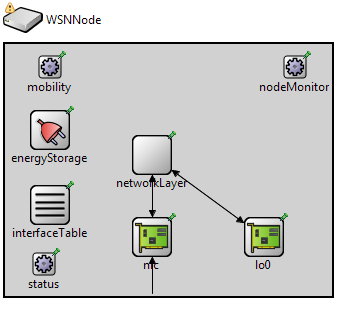
\includegraphics[scale=1]{\ImgPath/framework/node.png} 
	\end{center}
	\caption{Węzeł sieci}
	\label{abstractNode}
\end{figure}
\FloatBarrier
	\item WSNSensorNode - dziedziczy po WSNNode oraz zawiera dodatkowo moduł generujący pakiety - WSNSensorApp. Jego głównym zadaniem jest generowanie kolejnych pakietów z danymi, które zostało zrealizowane za pomocą funkcji \textit{sendPacket()}:
\begin{minted}[linenos]{cpp}
void WSNSensorApp::sendPacket()
{
    char msgName[32];
    sprintf(msgName, "%s-appData-%d",
        getParentModule()->getName(), numSent);

    cPacket *payload = new cPacket(msgName);
    payload->setByteLength(
        packetLengthPar->longValue());

    L3Address destAddr = chooseDestAddr();

    IL3AddressType *addressType =
        destAddr.getAddressType();
    INetworkProtocolControlInfo *controlInfo =
        addressType->createNetworkProtocolControlInfo();
    controlInfo->setDestinationAddress(destAddr);
    controlInfo->setTransportProtocol(protocol);
    payload->setControlInfo(
        check_and_cast<cObject *>(controlInfo));

    EV_INFO << "Sending packet: ";
    printPacket(payload);
    emit(sentPkSignal, payload);
    send(payload, "appOut");
    numSent++;
}
\end{minted}
W liniach 7-9 odbywa się wygenerowanie nowego pakietu z danymi. Wielkość danych odczytywana jest z parametru konfiguracyjnego \textit{packetLengthPar}. Linie 11-20 przedstawiają z kolei ustawienie odbiorcy pakietu (stacji bazowej) oraz protokołu transportowego.
	\begin{figure}[!htbp]
	\begin{center}
		\centering
		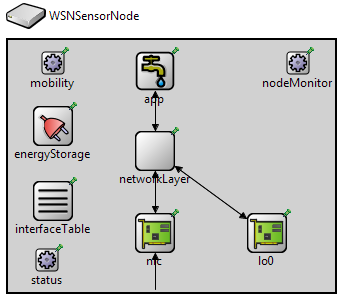
\includegraphics[scale=1]{\ImgPath/framework/sensor.png} 
	\end{center}
	\caption{Czujnik}
	\label{openlayers}
\end{figure}
\FloatBarrier
	\item WSNSinkNode - dziedziczy po WSNNode oraz zawiera dodatkowo moduł akceptujący pakiety od czujników o nazwie WSNSinkApp. Jego dodatkowym zadaniem jest wysłanie wiadomości z adresem stacji bazowej do węzłów czujnikowych na etapie inicjalizacji sieci. Za ten proces odpowiedzialna jest funkcja \textit{sendSinkInfo()}:
\begin{minted}{cpp}
void WSNSinkApp::sendSinkInfo() {
    char msgName[32];
    sprintf(msgName, "Sink address broadcast");

    SinkInfo *msg = new SinkInfo(msgName);
    msg->setByteLength(MAC_ADDRESS_SIZE);
    msg->setAddress(myAddr);
    msg->setKind(P_SinkInfo);

    L3Address destAddr = MACAddress::BROADCAST_ADDRESS;
    sendPacket(msg, destAddr);
}
\end{minted}
	\begin{figure}[!htbp]
	\begin{center}
		\centering
		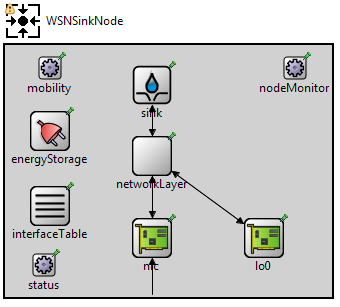
\includegraphics[scale=1]{\ImgPath/framework/sink.png} 
	\end{center}
	\caption{Stacja bazowa}
	\label{abstractNode}
\end{figure}
\FloatBarrier
	\item NodeCounter - moduł liczący działające węzły w sieci. Poniższy listing zawiera jego konfigurację w języku NED.
	\begin{minted}[linenos]{text}
simple NodeCounter
{
    parameters:
        @display("i=block/cogwheel;is=s");
        int numSensors;
        @signal[sinkDown](type=simtime_t);
        @signal[firstNodeDown](type=simtime_t);
        @signal[aliveNodesChanged];
        @statistic[aliveNodes]
            (title="Number of alive nodes";
            source=aliveNodesChanged; record=vector;
            interpolationmode=sample-hold);
        @statistic[sinkDownTime]
            (title="Sink shutdown time";
            source=sinkDown; unit=s; record=last;
            interpolationmode=none);
        @statistic[firstNodeDownTime]
            (title="First node shutdown time";
            source=firstNodeDown; unit=s; record=last;
            interpolationmode=none);
}
	\end{minted}
Linie 6-8 stanowią deklaracje sygnałów emitowanych przez moduł na potrzeby statystyczne:
\begin{itemize}
\item sinkDown - emitowany w momencie wyłączenia stacji bazowej w wyniku zbyt niskiego poziomu energii
\item firstNodeDown - emitowany w momencie pierwszej dezaktywacji węzła sieci
\item aliveNodesChanged - emitowany gdy liczba aktywnych węzłów ulegnie zmianie
\end{itemize}
	\item VolatileStateBasedEnergyConsumer - moduł pobierający energię w zależności od ustawionego stanu z możliwością dynamicznej zmiany poboru mocy.
	\begin{minted}{cpp}
void VolatileStateBasedEnergyConsumer::receiveSignal(
  cComponent *source, simsignal_t signalID,
  double value, cObject *details)
{
  transmitterTransmittingPowerConsumption =
      baseConsumption + mW(value);
  ...
}
	\end{minted}
\end{itemize}
\section{Protokoły}\label{sec:protocols}
Każda implementacja wybranego algorytmu trasowania wymaga stworzenia dwóch modułów. Jeden z nich dziedziczy po SimpleNetworkLayer, a drugi po NetworkProtocolBase.

Głównymi funkcjami, które jednocześnie wywoływane są przez silnik symulacji są handleSelfMessage, handleUpperPacket oraz handleLowerPacket.

\begin{minted}{cpp}
    virtual void handleSelfMessage(cMessage *msg) override;

    virtual void handleUpperPacket(cPacket *) override;

    virtual void handleLowerPacket(cPacket *) override;
\end{minted}

Do najprostszych protokołów trasowania należy Flood, więc do jego implementacji wykorzystany został istniejący już moduł z biblioteki INET. Należało jedynie utworzyć  moduł będący warstwą sieciową, a następnie skonfigurować go, aby wykorzystywał moduł Flood z biblioteki INET.
\subsection{SPIN}
Protokół SPIN został zaimplementowany zgodnie z zaproponowanym w artykule \cite{Kulik2002} wariancie SPIN-RL.

Kod odpowiadający za logikę protokołu znajduje się w klasie SPIN, która dziedziczy po klasie NetworkProtocolBase oraz implementuje interfejs INetworkProtocol z biblioteki INET.

\begin{minted}{cpp}
class SPIN : public NetworkProtocolBase,
    public INetworkProtocol
\end{minted}

Moduł po otrzymaniu pakietu z wyższej warstwy za pomocą funkcji \textit{isNegotiationViable()} dokonuje decyzji, czy węzeł ma dostatecznie dużo energii, aby przeprowadzić negocjację. W przypadku pozytywnej decyzji rozpoczynany jest proces negocjacji. W przeciwnym wypadku dane rozgłaszane są bezpośrednio, z pominięciem negocjacji funkcją \textit{simpleSend(msg)} z linii 10. Całość procesu przetwarzania pakietów z wyższej warstwy obrazuje poniższy fragment kodu.

\begin{minted}[linenos]{cpp}
void SPIN::handleUpperPacket(cPacket *m)
{
    SPINDatagram *msg = encapsMsg(m, DATA);
    msg->setSeqNum(seqNum);
    seqNum++;

    if (isNegotiationViable()) {
        advertiseData(msg);
    } else {
        simpleSend(msg);
    }
    nbDataPacketsSent++;
}
\end{minted}

Teoretyczny opis protokołu SPIN nie zawiera algorytmu, który węzły powinny wykorzystywać przy podejmowaniu decyzji czy rozpoczęcie procesu negocjacji jest zasadne z punktu widzenia oszczędnego korzystania z zasobów energetycznych. W implementacji zaproponowany więc został algorytm wykorzystujący funkcję prawdopodobieństwa o poniższym wzorze ogólnym:
\[
	f(x) = \frac{k*x}{k - x + 1}, x \in <0, 1>
\]

\begin{figure}[H]
	\begin{center}
		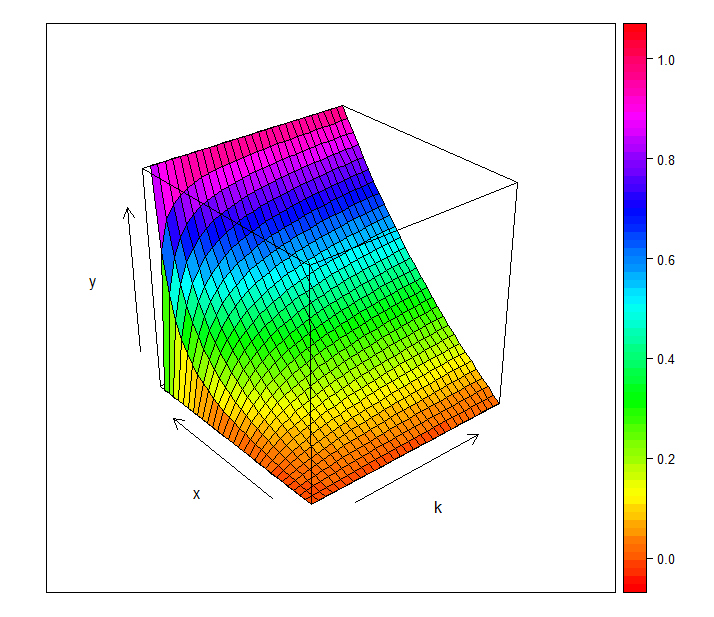
\includegraphics[scale=0.8]{\ImgPath/charts/prob_function_gen.png}
	\end{center}
	\caption{Wykres funkcji prawdopodobieństwa dla $x \in <0, 1>$ i $k \in <0, 2>$}
\end{figure}

Jako parametr k przyjęte zostało 1,2, a jako zmienną x stosunek aktualnej energii węzła do jego energii maksymalnej. Po podstawieniu otrzymuje się poniższy wzór, który został wykorzystany bezpośrednio w implementacji: 

\[
	f(E_{akt}, E_{max}) = \frac{1.2 * \frac{E_{akt}}{E_{max}}}{1.2 - \frac{E_{akt}}{E_{max}} + 1}
\]

\begin{figure}[H]
	\begin{center}
		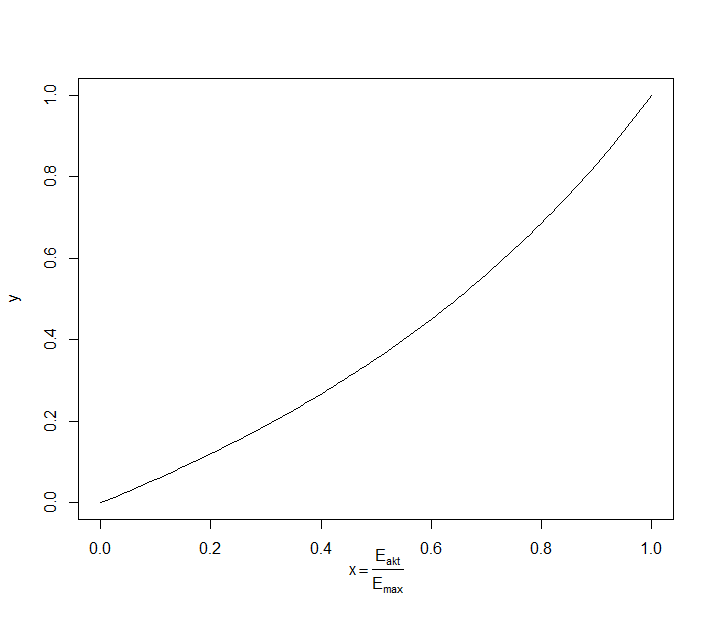
\includegraphics[scale=0.8]{\ImgPath/charts/prob_function_set_k.png}
	\end{center}
	\caption{Wykres funkcji prawdopodobieństwa dla $x \in <0, 1>$ i $k = 1.2$}
\end{figure}
Algorytm decyzyjny przedstawiony jest na poniższym listingu. Z przedziału [0, 1] losowana jest liczba, która następnie porównywana jest z wartością wcześniej opisanej funkcji. Jeżeli wylosowana liczba jest od niej mniejsza, podejmowana jest pozytywna decyzja o podjęciu negocjacji.
\begin{minted}{cpp}
bool SPIN::isNegotiationViable()
{
    double randomNumber = uniform(0, 1);
    double k = -1.2;
    double currentEnergyFrac = currentEnergy / maxEnergy;

    return randomNumber < (k*currentEnergyFrac / (k -
        currentEnergyFrac + 1));
}
\end{minted}
\subsection{LEACH i jego warianty}
Implementacja protokołu LEACH została wykonana na bazie istniejącej implementacji z symulatora Castalia. Pomimo zbieżności w architekturze silnika
symulacyjnego (Castalia oparta została na \omnetpp) konieczne było wprowadzenie szeregu zmian i poprawek.


W ALEACH zmieniony został sposób wyboru lokalnego węzła bazowego. W implementacji wykorzystany został mechanizm dziedziczenia. Klasa ALEACH stanowi rozszerzenie wcześniej zaimplementowanej klasy LEACH. Jedyną zmianą jest przesłonięcie funkcji \textit{selectCH} za pomocą tej zdefiniowanej na listingu poniżej, która realizuje założenia zawarte w akapicie \nameref{para:aleach} zawartym w podrozdziale \ref{subsec:leach}.
\begin{minted}{cpp}
void ALEACH::selectCH()
{
    ...
    double generalProb = (double)expectedCHNum / 
        (double)(numSensors - expectedCHNum * 
            (roundNumber % (numSensors / expectedCHNum) ));
    double currentEnergy = 
        energyStorage->getResidualCapacity().get();
    double currentStateProb = (currentEnergy / maxEnergy) *
        ((double) expectedCHNum / numSensors);
    ...
}
\end{minted}

Protokół Leach DCHS zaimplementowany został w sposób analogiczny do protokołu ALEACH.
\begin{minted}{cpp}
void LEACH_DCHS::selectCH()
{
   ...
   probability = percentage / (1 - percentage * (roundNumber
       % (int)(1/percentage)))
       * (currentEnergy / maxEnergy +
       (notCHRounds / (1/percentage))
       * (1 - (currentEnergy / maxEnergy)));
   ...
}
\end{minted}
\section{Poprawa biblioteki INET}
Biblioteka INET jest aktywnie rozwijana oraz poprawiana. Jednakże część biblioteki implementująca moduły związane z sieciami czujnikowymi oraz sieciami typu BAN są zdecydowanie rzadziej aktualizowane. W ramach niniejszej pracy został stworzony szereg dedykowanych poprawek dla projektu:

\paragraph{RSSI} Biblioteka INET nie udostępnia warstwie sieciowej RSSI, którego wartość jest niezbędna w implementacji protokołów LEACH. Problem został już wcześniej zasygnalizowany przez jednego z użytkowników, jednakże nie został on rozwiązany. W ramach pracy powstała poprawka udostępniająca ten parametr.

\begin{minted}{diff}
cPacket *CSMA::decapsMsg(CSMAFrame *macPkt)
{
+   ReceptionIndication *cInfo =
+     check_and_cast<ReceptionIndication *>
+     (macPkt->removeControlInfo());
+   double rssi = cInfo->getRSSI().get();
    cPacket *msg = macPkt->decapsulate();
-   setUpControlInfo(msg, macPkt->getSrcAddr());
+   setUpControlInfo(msg, macPkt->getSrcAddr(), rssi);

    return msg;
}

/**
 * Attaches a "control info" (MacToNetw) structure (object)
 * to the message pMsg.
 */
- cObject *CSMA::setUpControlInfo(cMessage *const pMsg,
-   const MACAddress& pSrcAddr)
+ cObject *CSMA::setUpControlInfo(cMessage *const pMsg,
+   const MACAddress& pSrcAddr, double rssi)
{
    SimpleLinkLayerControlInfo *const cCtrlInfo =
      new SimpleLinkLayerControlInfo();
    cCtrlInfo->setSrc(pSrcAddr);
+   cCtrlInfo->setRssi(rssi);
    pMsg->setControlInfo(cCtrlInfo);
    return cCtrlInfo;
}
\end{minted}

\paragraph{Dodanie możliwości zmiany modułu MAC w Ieee802154NarrowbandNic} W pierwotnej wersji rodzaj modułu MAC został zdefiniowany w sposób nie umożliwiający jego zmiany. Poprawka polega na wykorzystaniu zmiennej do przechowywania nazwy modułu MAC, który ma zostać dodany.
\begin{minted}{diff}
module Ieee802154NarrowbandNic like IWirelessNic
{
    parameters:
        string interfaceTableModule;
        string radioType =
          default("Ieee802154NarrowbandScalarRadio");
+       string macType = default("Ieee802154NarrowbandMac");
        *.interfaceTableModule =
          default(absPath(interfaceTableModule));
        @display("i=block/ifcard");
    gates:
        input upperLayerIn;
        output upperLayerOut;
        input radioIn @labels(IRadioFrame);
    submodules:
-       mac: Ieee802154NarrowbandMac {
+       mac: <macType> like IMACProtocol {
            parameters:
                @display("p=100,150");
        }
 ...
}
\end{minted}

\paragraph{Poprawa modułu IPvXTrafGen, tak aby prawidłowo zachowywał się podczas deaktywacji węzła} Klasa implementująca moduł IPvXTrafGen dziedziczyła po klasie cSimpleModule, która nie wchodzi bezpośrednio w skład biblioteki INET (jest częścią \omnetpp). W związku z tym nie zostały w niej zaimplementowane funkcje związane z aktywnością węzła. Problem ten został naprawiony poprzez dokonanie zmiany rodzica klasy IPvXTrafGen na klasę ApplicationBase z biblioteki INET. Stanowi ona bazę dla klas implementujących zachowania modułów prostych należących do warstwy aplikacji. Udostępnione zostały również dzięki temu interfejsy związane z aktywacją oraz dezaktywacją węzła sieci.

\begin{minted}{diff}
- class INET_API IPvXTrafGen : public cSimpleModule,
-   public ILifecycle
+ class INET_API IPvXTrafGen : public ApplicationBase
{
  protected:
    enum Kinds { START = 100, NEXT };
@@ -69,13 +70,15 @@ class INET_API IPvXTrafGen :
@@    public cSimpleModule, public ILifecycle

    virtual int numInitStages() const override
      { return NUM_INIT_STAGES; }
    virtual void initialize(int stage) override;
-   virtual void handleMessage(cMessage *msg) override;
+   virtual void handleMessageWhenUp(cMessage *msg) override;
    virtual void refreshDisplay() const override;
    virtual void startApp();

    virtual void printPacket(cPacket *msg);
    virtual void processPacket(cPacket *msg);
-   virtual bool handleOperationStage(
-     LifecycleOperation *operation, int stage,
-     IDoneCallback *doneCallback) override;
+    virtual bool handleNodeStart(
+      IDoneCallback *doneCallback) override;
+    virtual bool handleNodeShutdown(
+      IDoneCallback *doneCallback) override;
+    virtual void handleNodeCrash() override;
\end{minted}

\paragraph{Uzupełnienie modułu CSMA o funkcje obsługujące jego wyłączenie oraz ponowne włączenie} Przed poprawką, wyłącznie się symulowanego węzła (w wyniku zużycia energii) powodowało wystąpienie wyjątku i awaryjne zakończenie symulacji.

\begin{minted}{cpp}
bool CSMA::handleNodeStart(IDoneCallback *doneCallback)
{
    macState = IDLE_1;
    return true;
}

bool CSMA::handleNodeShutdown(IDoneCallback *doneCallback)
{
    cancelEvent(backoffTimer);
    cancelEvent(ccaTimer);
    cancelEvent(sifsTimer);
    cancelEvent(rxAckTimer);
    macState = IDLE_1;
    for (auto & elem : macQueue) {
        delete (elem);
    }
    flushQueue();
    return true;
}

void CSMA::handleNodeCrash()
{
    cancelEvent(backoffTimer);
    cancelEvent(ccaTimer);
    cancelEvent(sifsTimer);
    cancelEvent(rxAckTimer);
    macState = IDLE_1;
    for (auto & elem : macQueue) {
        delete (elem);
    }
    clearQueue();
}
\end{minted}

\paragraph{Obsługę przypadku, gdy pakiet dociera do wyłączonego już węzła} Dodana została obsługa przypadku brzegowego, w którym węzeł zostawał wyłączony podczas odbioru transmisji pakietu.
\begin{minted}{cpp}
bool Radio::handleNodeShutdown(...) {
    ...
    if (receptionTimer && receptionTimer->isScheduled())
        abortReception(receptionTimer);
    ...
}
\end{minted}